\documentclass[../_main/handlingar.tex]{subfiles}
\begin{document}
\motion{Förbättrad förvaring för sektionens lager}
Lagerutrymmet i våra lokaler är inte optimalt och vi ser möjligheter till förbättring för att förvara sektionens saker. I Pump är det svårt att komma åt all servis, glas osv då det ibland inte går att öppna skåpsdörrar på grund av allt som förvaras där inne. Vårt förslag är att byta ut skåpen mot nya hyllor som inte har dörrar och vi vill flytta frysen till en smartare lösning för att få in ytterligare en hylla. På så sätt får vi tre hyllor istället för två. (Se bifogad ritning)

Detsamma gäller i CM. Läsken står mitt på golvet och detta leder till att det blir mindre plats att röra sig på. Komma in? Vi kommer knappt ut! Här anser vi också att nya hyllor längs med väggarna optimerar förvaringsutrymmet.

\begin{center}
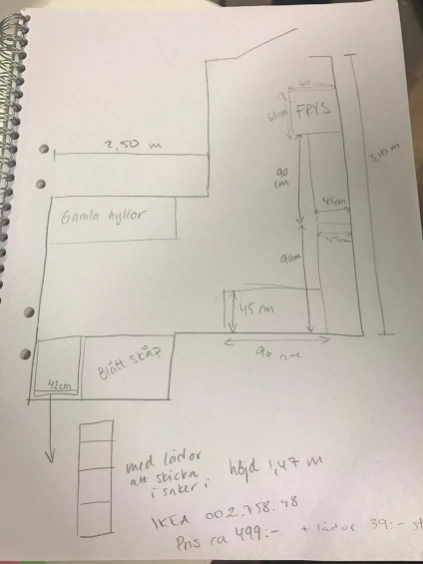
\includegraphics[width=7cm,height=8cm]{lager.png}
\end{center}

Med detta i beaktelse yrkar motionärerna på:
\begin{attsatser}
    \att köpa in fyra paket förvaringshyllor, dvs åtta hyllor totalt, till CM och Pump (4 á 600 kr).
    \att köpa in en smal, hög hylla till Pump med lådor (655 kr).
    \att budgeten för projektet sätts till 4000 kr för att också täcka transportkostnader.
    \att kostnaden belastar utrustningsfonden.
    \att detta läggs på beslutsuppföljningen till HT/17 där undertecknad står som ansvarig.
\end{attsatser}
\begin{signatures}{2}
    \mvh
    \signature{Sanna Nordberg}{Hovmästare}
    \signature{Matilda Dahlström}{Hovmästare}
\end{signatures}

\end{document}
